\section{Advanced SS Configuration Settings and Advice}

\hypertarget{TVpara}{}
\subsection{Using Time-Varying Parameters}

\hypertarget{tvOrder}{}
\subsubsection{Time-Varying Parameters in SS}

In SS v.3.30, mortality-growth, stock-recruitment (some parameters only, see \hyperlink{tv-sr}{ime-Varying Stock-Recruitment Considerations}, catchability, and selectivity base parameters can be time varying. Note that as of SS v. 3.30.16, time-varying parameters cannot be used with tagging parameters. There are 4 types of time-varying parameters in Stock Synthesis:
\begin{enumerate}
    \item Environmental Linkages: Links the base parameter with environmental data.
	\item Parameter deviations: Creates annual deviations from the base parameter during a user-specified range of years.
	\item Time blocks: The base parameter is changed during a "block" (or "blocks") of time (i.e., one or more consecutive years) in a way as specified by the user.
	\item Trends: A trend is applied to the parameter. Trends are specified using the same input columns as time blocks, but with different codes.
\end{enumerate}

Environmental linkages, parameter deviations, and either time blocks or trends can be applied to the same base parameter. SS processes each time-varying parameter specification and creates a time-series of parameter values that are used as SS subsequently loops through years.

%Note: tv_parameter_description contains \subsubsection{Specification of Time-Varying Parameters} 
\subsubsection{Specification of Time-Varying Parameters: Long Parameter lines} 

Time-varying specifications for a parameter are invoked elements 8 - 14 in the \hyperlink{paraOrder}{long parameter line setup}. Each element and the options for selection related to time-varying parameters are as described below.

\hypertarget{EnvVar}{}
\begin{itemize}

\item Environmental Link and variable (env\_var\&link; element 8)

	\begin{itemize}
	   \item The environmental link and variable input is two inputs specified using a single three digit number. The hundreds place contains the option for the link function, while the tens and ones place is used to specify the environmental variable or derived quantity to which the parameter is linked. If the environmental link and variable input is positive, then the parameter is linked to a variable specified in the data file environmental data; if it is negative, then the parameter is linked to a derived quantity. For example, env\_var\&link input 103 would use link type 1 and apply it to environmental data column 3, while the input -103  would use link type 1 and apply it to the "-3" column which is ln(relative summary biomass).
	   \item The link function options (hundreds place) for the env\_var\&link input are:
	   \begin{itemize}
	       \item 1 = exponential scalar: $P_{y} = P_{base}e^{P_{t}E_{y}}$
		   \item 2 = linear offset: $P_{y} = P_{base} + P_{t}E_{y}$
		   \item 3 = Bounded replacement: $P_{y} = min(P_{base})+\frac{max(P_{base})-min(P_{base})}{1+e^{P_tE_y+ln((P_{base}-min(P_{base})+0.0000001)/(max(P_{base})-P_{base}+0.0000001))}}$
		   \item 4 = Logistic: $P_{y} = P_{base}\frac{2}{1+e^{-P_{t2}(E_{y}-P_{t1})}}$
	   \end{itemize}
		where:
	   \begin{itemize}
	       \item $P_{y}$ = Parameter value in year $y$
           \item $P_{base}$ = Base parameter value
           \item $P_{t}$ = Time-varying parameter value
           \item $P_{t1}$ = First of 2 time-varying parameters (offset)
           \item $P_{t2}$ = Second of 2 time-varying parameters (slope)
           \item $E_{y}$ = Environmental index value or derived quantity value in year $y$
           \item $min(P_{base})$ = the minimum parameter bound of base parameter
           \item $max(P_{base})$ = the maximum parameter bound of base parameter
        \end{itemize}
		\item The variable options (tens and ones place, or $E_{y}$) for the env\_var\&link input are 1) a positive integer from 1 to 99 referencing a user input index time-series located in the \hyperlink{env-dat}{environmental data section} of the data file, or 2) a negative value of -1 to -4 where the index is represented by one of the following model-derived quantities:
		\begin{itemize}
			\item -1;  for ln(relative spawning biomass)
			\item -2;  for recruitment deviation
			\item -3;  for ln(relative summary biomass) (e.g., current year summary biomass divided by the unfished summary biomass)
			\item -4;  for ln(relative summary numbers)
		\end{itemize}
		\item The four derived quantities are all calculated at the beginning of each year within the model, so they are available inside SS to use as the basis for time-varying parameter links without violating any order of operations rules.
	\end{itemize}
	
\item Deviation Link (element 9). This must be specified if using parameter deviations, but otherwise should be left as 0. Link options for parameter deviations are:
	\begin{itemize}
		\item 1 = multiplicative: $P_y = P_{base}e^{\text{dev}_y*\text{dev}_{se}}$,
		\item 2 = additive: $P_y = P_{base} + \text{dev}_y*\text{dev}_{se}$,
		\item 3 = random walk. random walk options are now implemented by using rho in the objective function. SS now expects the estimated deviations to be normal in distribution and the deviation values are multiplied by the standard error parameter as they are used
		\item 4 = zero reverting random walk with rho. The deviation parameter is multiplied by the standard error parameter, rather than deviations being penalized according to a specified standard error (the approach in SS v.3.24)
		\item 5 = zero reverting random walk with rho and a logit transformation to stay within the minimum and maximum parameter bounds (approach added in SS v.3.30.16)
		\item 6 = mean reverting random walk with penalty to keep rmse near 1.0
		\item The option of applying the final model year deviation value into the forecast period was added in v. 3.30.13.  This new option is specified by selecting the appropriate deviation link option (1, 2, 3, or 4) and appending a 2 at the front (21, 22, 23, or 24) which will use the final year deviation value for all forecast years
	\end{itemize}
	where: 
	\begin{itemize}
	     \item $P_{y}$ = Parameter value in year $y$
         \item $P_{base}$ = Base parameter value
		 \item $\text{dev}_y$ is the deviation in year $y$
		 \item $\text{dev}_{se}$ is the standard error of the deviation
	\end{itemize}
\item Deviation Minimum Year (element 10)
	\begin{itemize}
		\item Year deviations start for parameter. This must be specified if using parameter deviations, but otherwise should be left as 0.
	\end{itemize}
	
\item Deviation  Maximum Year (element 11)
	\begin{itemize}
		\item Year deviations end for parameter. This must be specified if using parameter deviations, but otherwise should be left as 0.
	\end{itemize}
	
\item Deviation Phase (element 12)
	\begin{itemize}
		\item integer, the phase in which the deviations for the parameter should be estimated. This must be specified if using parameter deviations, but otherwise should be left as 0.
		%is there a recommended phase to use if wanting to estimate devs?
	\end{itemize}
	
\item Use Time Blocks or Trends (element 13). Time blocks and trends are both specified using this input. If neither are used, this should be left as 0. For trend options, the cumulative normal distribution function is used in all cases, but the parameterization differs.
	\begin{itemize}
		\item >0: time block index for parameter.
		\item -1: Offset option. Three parameters are estimated: end trend parameter value logistic offset, inflection year logistic offset, and width (i.e., the standard deviation of the cumulative normal function). Trend with final parameter value and year as offset from base parameter/base year. Offset trend value is in natural log space. Inflection year is also in natural log space and offset from ln(0.5). Width is directly specified.
		\item -2: Direct input option. Three parameters are estimated: end trend parameter value, inflection year, and width (i.e., the standard deviation of the cumulative normal function). Trend with final parameter value and year directly input. Width is directly input.
		\item -3: Fractional option. Three parameters will be estimated: end trend parameter value as a fraction of base parameter maximum - minimum, inflection year as a fraction of end year - start year, and width (i.e., the standard deviation of the cumulative normal function). Width is directly input.
	\end{itemize}
	
\item Time Block Functional Form (element 14). Leave as 0, unless time blocks are used.
	\begin{itemize}
		\item 0: multiplicative parameter ($P_{block} = P_{base}*e^{P_t}$)
		\item 1: additive parameter ($P_{block} = P_{base} + P_t$)
		\item 2: replace parameter ($P_{block} = P_t$)
		\item 3: random walk across blocks ($P_{block} = P_{block,-1} + P_t$)
		\item 4: mean reverting random walk
	\end{itemize}
	where:
	\begin{itemize}
        \item $P_{block}$ = Final parameter value in time block $block$
        \item $P_{base}$ = Base parameter value
		\item $P_{t}$ = Time-varying parameter value for a time block
		\item $P_{block,-1}$ = Final parameter value in the previous time block
     \end{itemize}
\end{itemize}


%\myparagraph{Block Trends}
%Note: the below equations just show the parameterization for option 1 of the block trends. I'm not sure how helpful this is, as it is written as C++ code. To make more useful, it should be rewritten as a mathematical equation.

%Additional information regarding the options for applying blocks (element 13):
%\begin{itemize} 
%	\item -1: Trend bounded by base parameter minimum maximum and parameters in transformed units (use with caution),
%	\begin{itemize}
%		\item Logistic approach to trend as offset from base parameter
%		\item Transform the base parameter from the parameter section:
%		\begin{equation}
%			\text{temp} = -0.5*ln\Bigg(\frac{\text{Parm}_{p,LB}-\text{p,Parm}_{UB}+0.0000002}{\text{Parm}_p-\text{Parm}_{p,LB}+0.0000001}-1\Bigg)
		%\end{equation}
		%\item Add the offset. Note, that offset values in in the transform space.
		%\begin{equation}
		%	\text{temp2} = \sum_{p=1}^{P}\text{TV parameter}{p}MGparm(k+1)
		%\end{equation}
		%\item Back transform
		%\begin{equation}
	%		\text{temp1} = \text{Parm}_{p,LB}+\frac{\text{Parm}_{p,UB}-\text{Parm}_{p,LB}}{1+e^{-2*\text{temp}}}
		%\end{equation}			
	%\end{itemize}
%\end{itemize}
	 
\subsubsection{Specification of Time-Varying Parameters: Short Parameter lines} 

If a time-varying specification set up in the long parameter lines for a particular sections requires additional parameters, short parameter lines need to be created following all the long parameter lines (unless \hyperlink{autogen}{autogeneration} is used, which creates short parameter lines upon running that model that are output in control.ss_new). The number of lines added depends on the time-varying parameter specification.

For example, if two parameters were specified to have environmental linkages in the MG parameter section, below the MG parameters would be two parameter lines (when not autogenerating these lines), which is an environmental linkage parameter for each time-varying base parameter:
\begin{longtable}{ p{0.7cm} p{0.7cm} p{0.7cm}  p{1cm}  p{1.4cm}  p{1cm} p{1cm} p{6.7cm}  }
	\hline
	   &    &      & Prior &  Prior & Prior & & \Tstrut\\
	LO & HI & INIT & Value &  SD    & Type  & Phase & Parameter Label \Bstrut\\
	\hline
	\endfirsthead
	
	\hline
	   &    &      & Prior &  Prior & Prior &  & \Tstrut\\
	LO & HI & INIT & Value &  SD    & Type  & Phase & Parameter Label \Bstrut\\
	\hline
	\endhead
	
	\endfoot
	
	\endlastfoot
	
	\multicolumn{7}{l}{COND: Only if MG parameters are time-varying} \Tstrut\\
	-99   & 99  & 1 & 0 & 0.01 & 0 & -1 &\#Wtlen\_1\_Fem\_ENV\_add\Tstrut\\
	-99   & 99  & 1 & 0 & 0.01 & 0 & -1 &\#Wtlen\_2\_Fem\_ENV\_add\Bstrut\\
	\hline
\end{longtable}

 In SS v.3.30, the time-varying input short parameter lines are re-organized such that all parameters that affect a base parameter are clustered together with time blocks (or trend) first, then environmental linkages, then parameter deviations. For example, if the mortality-growth (MG) base parameters 3 and 7 had time varying changes, the order would look like:

\begin{center}
	\begin{longtable}{p{5cm} p{10cm}}
		\hline
		MG base parameter 3 & Block parameter 3-1\Tstrut\\
		& Block parameter 3-2\\
		& Environmental link parameter 3-1\\
		& Deviation se parameter 3 \\
		& Deviation rho parameter 3 \Bstrut\\
		MG base parameter 7 & Block parameter 7-1 \\
		& Deviation se parameter 7 \\
		& Deviation rho parameter 7 \Bstrut\\
		\hline	 	                    
		
	\end{longtable}
\end{center}

The number of short parameter lines for each time-varying setup selected depends on the selection options. The autogen feature can be used to figure out which parameter lines are needed. The short parameter lines needed for different time-varying options are:

\begin{itemize}
    \item Environmental Linkages: Requires 1 short parameter line ($P_{t}$), except for option 4, which requires 2 short parameter lines ($P_{t1}$ and $P_{t2}$).
    \item Parameter deviations: Requires 2 short parameter lines, one for the standard error ($\text{dev}_{se}$), followed by one for rho. Rho is required input, but only used with random walk options (Rho can be set at 1 for a random walk with no drift or >1 for a random walk with drift).
    \item Time Blocks: One parameter for each time block ($P_{t}$) set up in the pattern.
    \item Trends: Requires 3 parameter lines. The interpretation of the parameters differs by the trend option selected, but in general they are a parameter for the final parameter value, a parameter for the inflection point year, and a parameter for the width.
\end{itemize}

\subsubsection{Example timevarying parameter setups}

The time-varying parameter options in Stock Synthesis are flexible. Below are some example setups that illustrate how the time-varying options could be used in a model, although there are many more possible setups.

\myparagraph{Environmental linkages}
  \begin{itemize}
    \item Suppose growth rate is found to be linked with an index of water temperature. The water temperature proxy could be input into the data file as environmental data. If it is input as parameter number 1, the growth parameter K (if using a von Bertalanfy growth equation) could be linked to this data by using the code "201" into the env\_var\&link function input. This would establish an offset link between the parameter and the temperature proxy. One additional parameter line will be required after the "MG parameter" long parameter lines section.
    \item Suppose selectivity is thought to shift depending on the population size; in this case, assume smaller fish are selected when there are lower population numbers. The selectivity parameter could be made time-varying using the code "-104" in the env\_var\&link option, which assumes a exponential scalar link between the base selectivity parameter and the time varying parameter value. One additional parameter line will be specified at the end of the selectivity long parameter lines section.
  \end{itemize}
\myparagraph{Parameter Deviations
  \begin{itemize}
    \item Suppose a selectivity parameter is thought to drift every year during 2000-2010 in a model. This could be represented using a random walk link option available within the parameter deviations options. To implement this, the user could input 3 into the "dev link" input on the long parameter line for the selectivity paramter, and then input values 2000 and 2010 for "dev min yr" and "dev max yr", respectively. The dev phase could be set to 3. With this setup, 2 additional short parameter lines would be expected, one for the standard error and one for rho. Both of these will be used since a random walk option is selected. To use a random walk without drift, rho is set at 1 with a negative phase.
  \end{itemize}
\myparagraph{Time Blocks}
  \begin{itemize}
    \item Offset approach: One or more time blocks are created and cover all or a subset of the years. Each block gets a parameter that is used as an offset from the base parameter (time block functional form 1). In this situation, typically the base parameter and each of the offset parameters are estimated. In years not covered by blocks, the base parameter alone is used.  However, if blocks cover all the years, then the value of the block parameter is completely correlated with the mean of the block offsets, so model convergence and variance estimation could be affected.  The recommended approach when using offsets is to not have all years covered by blocks, or to fix the base parameter value at a reasonable level when doing offsets for all years.	
	\item Replacement approach, Option A: Here time blocks are created which cover a subset of the years.  The base parameter is used in the non-block years and the value of that base parameter is replaced by the block parameter in each respective block (time block functional form 2). In this situation, typically the base parameter and each of the block parameters are estimated.	
	\item Replacement approach, Option B: Here replacement time blocks are created for all the years.  In this case the base parameter is simply a placeholder that is always replaced by a block parameter (time block functional form 2). In this situation, do not allow SS to estimate the base parameter and only estimate the corresponding block replacement parameters, otherwise, the search algorithm will be attempting to estimate parameters that do not contribute to the log likelihood, so model convergence and variance estimation could be affected.  Note however, that the minimum and maximum for the base parameter are used as checks on the minimum and maximum of the blocks.
  \end{itemize}
\myparagraph{Trends}
  \begin{itemize}
    \item Suppose natural mortality was thought to increase from 0.1 to 0.2 during 2000 to 2010. This could be input as a trend. First, the natural mortality parameter would be fixed at an initial value of 0.1. Then, a value of -2 could be input into the "use block" column of the natural mortality long parameter line to indicate that the direct input option for trends should be used. The long parameter line for M could look like:
	\begin{center}
	\begin{longtable}{p{1cm} p{1cm} p{1cm}  p{1.5cm}  p{3cm}  p{2cm}  p{3.5cm}  }
		
		\hline
		LO \Tstrut & HI & INIT & <other entries> & PHASE & <other entries> & Use_Block & Block Fxn & Parameter Label\Bstrut\\
		\hline
		0          & 4 & 0.1 &  \multicolumn{1}{c}{...} & -1 & \multicolumn{1}{c}{...} & -2 & 0 & \#M \Bstrut\\
		\hline
	\end{longtable}
    \end{center}
	Three short parameter lines are then expected after the mortality-growth long parameter lines, one for the final value, one for the inflection year and one for the width. The final value could be fixed by using 0.2 as the final value on the short parameter line and a negative phase value. The inflection year could be fixed at 2005 by inputting 2005 for the inflection year in the short parameter line with a negative phase. Finally, the width value (i.e., standard deviation of the cumulative normal distribution) could be set at 3 years. The short parameter lines could look like:
	begin{longtable}{ p{0.7cm} p{0.7cm} p{0.7cm}  p{1cm}  p{1.4cm}  p{1cm} p{1cm} p{6.7cm}  }
	\hline
	   &    &      & Prior &  Prior & Prior & & \Tstrut\\
	LO & HI & INIT & Value &  SD    & Type  & Phase & Parameter Label \Bstrut\\
	\hline
	\endfirsthead
	
	\hline
	   &    &      & Prior &  Prior & Prior &  & \Tstrut\\
	LO & HI & INIT & Value &  SD    & Type  & Phase & Parameter Label \Bstrut\\
	\hline
	\endhead
	
	\endfoot
	
	\endlastfoot
	
	\multicolumn{7}{l}{COND: Only if MG parameters are time-varying} \Tstrut\\
	0.001 & 4    & 0.2  & 0 & 0.01 & 0 & -1 &\#M\_TrendFinal\Tstrut\\
	1999  & 2011 & 2005 & 0 & 0.01 & 0 & -1 &\#M\_TrendInfl\Bstrut\\
	-99   & 99   & 3    & 0 & 0.01 & 0 & -1 &\#M\_TrendWidth_yrs\Bstrut\\
	\hline
    \end{longtable}
\end{itemize}



\hypertarget{tvgrowth}{}
\subsubsection{Time-Varying Growth Considerations}
When time-varying growth is used, there are some additional considerations to be aware of:
\begin{itemize}
	\item Growth in the forecast with time blocks: Growth deviations propagate into the forecast. The user can select which growth parameters get used during the forecast by setting the end year of the last block, if using time blocks. If the last block ends in the model's end year, then the growth parameters in effect during the forecast will be the base parameters.  By setting the end year of the last block to one year past the model end year (endyr), the model will continue the last block's growth parameter levels throughout the forecast.
	\item The equilibrium benchmark quantities (MSY, F40\%, etc.) previously used the model end year's (endyr) body size-at-age, which is not in equilibrium. Through the forecast file, it is possible to specify a range of years over which to average the size-at-age used in the benchmark calculations.
	% Which input in forecast?? The benchmark years input? I couldn't find this option...
\end{itemize}

\hypertarget{tv-sr}{}
\subsubsection{Time-Varying Stock-Recruitment Considerations}
\begin{itemize}
	
	\item The $\sigma_R$ and autocorrelation parameters can not be time-varying. 
	% Is this true? Or can they be time varying but it is not advisable because it doesn't make much sense?
	
	\item The autocorrelation parameter cannot be estimated accurately within SS \citep{johnson_can_2016}, so external (i.e., external to SS) estimation for selecting an autocorrelation value is currently recommended. 
		
	\item The value of R0 and steepness in the initial year are used within virgin calculations and within the benchmarks for calculation of the denominator in depletion estimates. The average value of R0 and steepness in the range of years specified as the benchmark years inputs 9 and 10 (see \hyperlink{fore-specify}{the forecast file specifications}) is used for MSY type calculations. 
	%So, for example, a long-term climate effect could cause R0 to change over time and B\textsubscript{MSY} could now be calculated for some future range of years.
	
	\item The spawner recruit regime parameter   S This regime shift parameter can have blocks, environmental links or random deviations. 
	
	\item The regime shift parameter line allows for multi-year or environmentally driven deviations from R0 without changing R0 itself. The regime shift base parameter is intended to have a base value of 0.0 and not be estimated. imilar to the cohort-growth deviation, it serves simply as a base for adding time-varying adjustments.
	
	\item The same algebraic effect on the calculated recruitment can be achieved by different combinations of spawner-recruit parameter options (e.g., changing R0 directly insead of the regime shift parameter). It is recommened to use block, trend or environmental effects on R0 only for long-term effects, and use time-vary effects on the regime shift parameter for transitory but multi-year deviations from R0.	
	
	\item If the R0 or steepness parameters are time-varying, then SS will use the current year's parameters to calculate recruits as a function of the spawning biomass. If the regime shift parameter is time-varying, then SS applies the change in the regime shift parameter \textbf{after} calculating recruits as a function of spawning biomass. The expected deviations can no longer be linked to "env": instead the environmental effect will be on the "regime". 
	%note: last sentence above is not clear and needs to be rewritten.

\end{itemize}

%No longer need details about 3.24, someone could reference an older manual if
%desired.

%In SS v.3.24 and before, only a short parameter line was used for the spawner-recruitment section. SS v.3.30 now requires long parameter lines in the spawner-recruitment section because it now uses the same time-varying parameter approach as the biology and selectivity parameters. This generic time-varying approach replaces the spawner recruit envlink concept in SS v.3.24.  Also, the R1 offset was effectively a block to implement a regime shift for the initial equilibrium year.  Now in v.3.30, the R1 offset parameter is replaced by a parameter termed "regime shift". 

%If a SS v.3.24 model implemented the R1 offset approach this can be mimicked in v.3.30 by the stock recruit regime parameter. For any given year, including startyr - 1, the R0 is replaced by $R0*exp(\mathrm{SR\_Regime}_y)$. So to mimic the R1\_offset, you need to put a block on SR\_regime for y = startyr - 1. But if SR\_regime has some change during your main time series, that change will be filtered through the stock-recruit relationship into an impact on the numbers at age for whatever years are impacted. This can also apply to the forecast. A block on SR\_regime is also easier than some of the old dummy environmental variables that were created in the past to adjust recruitment up and down for long periods.



% Question: any particular details needed for q or selectivity tv params?
% Add sections if so.

\subsubsection{Forecast Considerations with Time-Varying Parameters}

Users should judiciously consider which parameter values are applied during forecast years. SS will default to use all base parameter values during the forecast period, but alternatively, which years of selectivity, relative F, and recruitment should be used during the forecast period by specifying in the \hyperlink{fore-specify}{forecast file}. 

% Any other additional details?

%\subsubsection{Time-Varying Parameter Change from Earlier SS Versions}
%The approach to time varying parameters was overhauled from SS v.3.24 to SS v.3.30. In SS v.3.24, the group of biology parameters (termed mortality-growth parameters) and the selectivity parameters used the same long parameter line approach, but each was implemented in its own section of the code. The spawner-recruitment parameters used short parameter lines and a different approach for linkage to an environmental variable and the R1 offset provided a limited type of block. The catchability parameters also used short parameter lines and had its own approach to doing environmental linkage and random deviations, but not blocks. Then finally, the tagging parameters had long parameter lines, but there was no code to interpret any time-varying info in those lines.

%%%%%%%%%%%%%%%%%%%%%%%%%%%%%%%%%%%%%%%%%%%%%%%%%%%%%%%%%%%%%%%%%%%%%%%%%%%%%%%%%%%%%%%%%%%%%%%%%%%%%%%%%%%%%%%%%%%%%
%%%%%%%%%%%%%%%%%%%%%%%%%%%%%%%%%%%%%%%%%%%%%%%%%%%%%%%%%%%%%%%%%%%%%%%%%%%%%%%%%%%%%%%%%%%%%%%%%%%%%%%%%%%%%%%%%%%%%
\hypertarget{2DAR}{}
\subsection{Parameterizing the Two-Dimensional Autoregressive Selectivity}
When the two-dimensional autoregressive selectivity feature is turned on for a fleet, the selectivity is calculated as a product of the assumed selectivity pattern and a non-parametric deviation term deviating from this assumed pattern:

\begin{equation}
\hat{S}_{a,t} = S_aexp^{\epsilon_{a,t}}
\end{equation}

where $S_a$ is specified in the corresponding age/length selectivity types section and it can be either parametric (recommended) or non-parametric (including any of the existing selectivity options in SS); $\epsilon_{a,t}$ is simulated as a two-dimensional first-order autoregressive (2D AR1) process:

\begin{equation}
vec(\epsilon) \sim MVN(\mathbf{0},\sigma_s^2\mathbf{R_{total}})
\end{equation}

where $\epsilon$ is the two-dimensional deviation matrix and $\sigma_s^2\mathbf{R_{total}}$ is the covariance matrix for the 2D AR1 process. More specifically, $\sigma_s^2$ quantifies the variance in selectivity deviations and $\mathbf{R_{total}}$ is equal to the kronecker product ($\otimes$) of the two correlation matrices for the among-age and among-year AR1 processes:

\begin{equation}
\mathbf{R_{total}}=\mathbf{R}\otimes\mathbf{\tilde{R}}
\end{equation}

\begin{equation}
\mathbf{R}_{a,\tilde{a}}=\rho_a^{|a-\tilde{a}|}
\end{equation}

\begin{equation}
\mathbf{\tilde{R}}_{t,\tilde{t}}=\rho_t^{|t-\tilde{t}|}
\end{equation}

where $\rho_a$ and $\rho_t$ are the among age and among year AR1 coefficients, respectively. When both of them are zero, $\mathbf{R}$ and $\mathbf{\tilde{R}}$ are two identity matrices and their Kronecker product, $\mathbf{R_{total}}$, is also an identity matrix. In this case selectivity deviations are essentially identical and mutually independent:

\begin{equation}
\epsilon_{a,t}\sim N(0,\sigma_s^2)
\end{equation} 

\myparagraph{Using the Two-Dimensional Autoregressive Selectivity}
Note, \citet{xu_new_2019} has additional information on tuning the 2D AR selectivity parameters. First, fix the two AR1 coefficients ($\rho_a$ and $\rho_t$) at 0 and tune $\sigma_s$ iteratively to match the relationship:

\begin{equation}
\sigma_s^2=SD(\epsilon)^2+\frac{1}{(a_{max}-a_{min}+1)(t_{max}-t_{min}+1)}\sum_{a=a_{min}}^{a_{max}}\sum_{t=t_{min}}^{t_{max}}SE(\epsilon_{a,t})^2
\end{equation}

The minimal and maximal ages/lengths and years for the 2D AR1 process can be freely specified by users in the control file. However, we recommend specifying the minimal and maximal ages and years to cover the relatively "data-rich" age/length and year ranges only. Particularly we introduce: 

\begin{equation}
b=1-\frac{\frac{1}{(a_{max}-a_{min}+1)(t_{max}-t{min}+1)}\sum_{a=a_{min}}^{a_{max}}\sum_{t=t_{min}}^{t_{max}}SE(\epsilon_{a,t})^2}{\sigma_s^2}
\end{equation}

as a measure of how rich the composition data is regarding estimating selectivity deviations. We also recommend using the Dirichlet-Multinomial method to "weight" the corresponding composition data while $\sigma_s$ is interactively tuned in this step.

Second, fix $\sigma_s$ at the value iteratively tuned in the previous step and estimate $\epsilon_{a,t}$. Plot both Pearson residuals and $\epsilon_{a,t}$ out on the age-year surface to check their 2D dimensions. If their distributions seems to be not random but rather be autocorrelated (deviation estimates have the same sign several ages and/or years in a row), users should consider estimating and then including the autocorrelations in $\epsilon_{a,t}$.

Third, extract the estimated selectivity deviation samples from the previous step for estimating $\rho_a$ and $\rho_t$ externally by fitting the samples to a stand-alone model written in Template-Model Builder (TMB). In this model, both $\rho_a$ and $\rho_t$ are bounded between 0 and 1 via applying a logic transformation. If at least one of the two AR1 coefficients are notably different from 0, SS should be run one more time by fixing the two AR1 coefficients at their values externally estimated from deviation samples. The Pearson residuals and $\epsilon_{a,t}$ from this run are expected to distribute more randomly as the  autocorrelations in selectivity deviations can be at least partially included in the 2D AR1 process.


%%%%%%%%%%%%%%%%%%%%%%%%%%%%%%%%%%%%%%%%%%%%%%%%%%%%%%%%%%%%%%%%%%%%%%%%%%%%%%%%%%%%%%%%%%%%%%%%%%%%%%%%%%%%%%%%%%%%%
%%%%%%%%%%%%%%%%%%%%%%%%%%%%%%%%%%%%%%%%%%%%%%%%%%%%%%%%%%%%%%%%%%%%%%%%%%%%%%%%%%%%%%%%%%%%%%%%%%%%%%%%%%%%%%%%%%%%%

\subsection{Continuous seasonal recruitment}
It is awkward in SS to set up a seasonal model such that recruitment can occur with similar and independent probability in any season of any year.  Consequently, some users have attempted to setup SS so that each quarter appears as a year.  They have set up all the data and parameters to treat quarters as if they were years (i.e., each still has a duration of 1.0 time step).  This can work, but requires that all rate parameters be re-scaled to be correct for the quarters being treated as years.

Another option is available.  If there is one season per year and the season duration is set to 3 (rather than the normal 12), then the season duration is calculated to be 3/12 or 0.25. This means that the rate parameters can stay in their normal per year scaling and this shorter season duration makes the necessary adjustments internally. Some other adjustments to make when doing quarters as years include:

\begin{itemize}
	\item Re-index all "year seas" inputs to be in terms of quarter-year because all are now season 1; increase end year (endyr) value in sync with this.
	\item Increase max age because age is now in quarters.
	\item In the age error definitions, increase the number of entries in accord with new max age
	\item In the age error definitions, recode so that each quarter-age gets assigned to the correct age bin. This is because the age data are still in terms of age bins; i.e., the first 4 entries for quarter-ages 1 through 4 will all be assigned to age bin 1.5; the next four to age bin 2.5;  you cannot accomplish the same result by editing the age bin values because the standard deviation of ageing error is in terms of age bin.
	\item In the control file, multiple the natural mortality age breakpoints and growth Amin and Amax values by 1/season duration.
	\item Decrease the R0 parameter starting value because it is now the average number of recruitments per quarter year.
	\item Edit the recruitment deviation (rec\_dev) start and end years to be in terms of quarter year.
	\item Edit any age selectivity parameters that refer to age to now refer to quarter age.
	\item If there needs to be some degree of seasonality to recruitment or some parameter, then you could create a cyclic pattern in the environmental input and make recruitment or some other parameter a function of this cyclic pattern.
\end{itemize}

A good test showing comparability of the 3 approaches to setting up a quarterly model should be done.

\pagebreak

%%%%%%%%%%%%%%%%%%%%%%%%%%%%%%%%%%%%%%%%%%%%%%%%%%%%%%%%%%%%%%%%%%%%%%%%%%%%%%%%%%%%%%%%%%%%%%%%%%%%%%%%%%%%%%%%%%%%%
%%%%%%%%%%%%%%%%%%%%%%%%%%%%%%%%%%%%%%%%%%%%%%%%%%%%%%%%%%%%%%%%%%%%%%%%%%%%%%%%%%%%%%%%%%%%%%%%%%%%%%%%%%%%%%%%%%%%%

\section{Detailed Information on SS Processes}

The processes and calculations with SS can be complex and not transparent based on the model input files. Here additional information is provided to users to assist in understanding some of these processes.

\subsection{Jitter}
\hypertarget{Jitter}{}
The jitter function has been updated with SS v.3.30.  The following steps are now performed to determine the jittered starting parameter values (illustrated in Figure \ref{fig:jitter}):
\begin{enumerate}
	\item A normal distribution is calculated such that the pr(P\textsubscript{MIN}) = 0.1\% and the pr(P\textsubscript{MAX}) = 99.9\%.
	\item A jitter shift value, termed "\textit{K}", is calculated from the distribution equal to pr(P\textsubscript{CURRENT}).
	\item A random value is drawn, "\textit{J}", from the range of \textit{K}-jitter to \textit{K}+jitter.
	\item Any value which falls outside the 0-1 range (in the cumulative normal space) is mapped back from the bound to a point one-tenth of the way from the bound to the initial value.
	\item \textit{J} is a new cumulative normal probability value.
	\item Calculate a new parameter value, P\textsubscript{JITTERED}, such that pr(P\textsubscript{JITTERED}) = \textit{J}.
\end{enumerate}

\begin{figure}[h]
	\begin{center}
		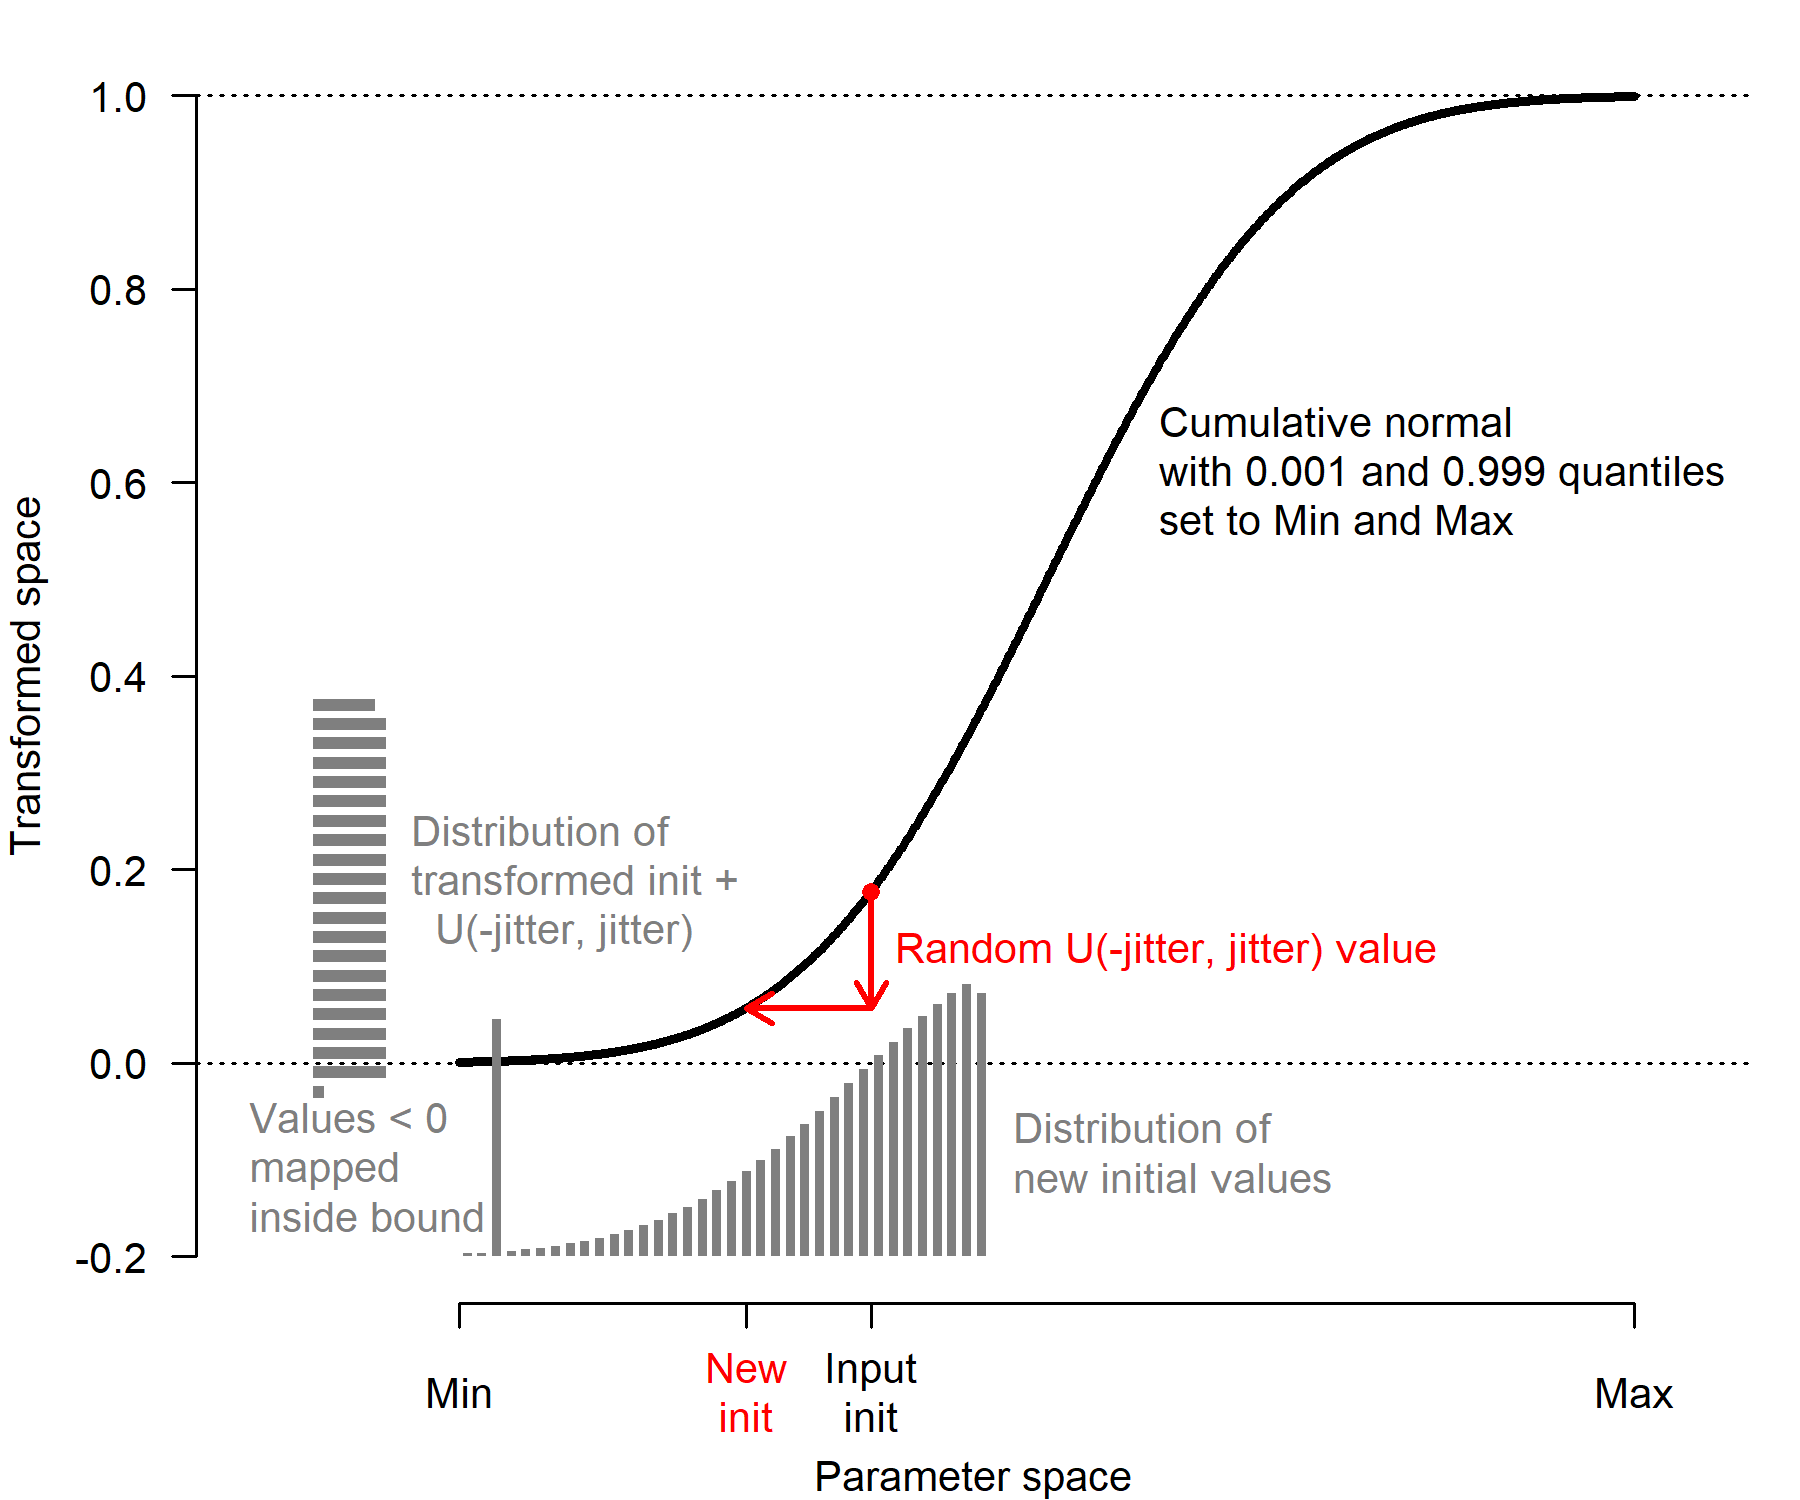
\includegraphics[scale = 0.75]{jitter_illustration}\\
		\caption{Illustration of the jitter algorithm}
		\label{fig:jitter}
	\end{center}
\end{figure}

In SS, the jitter fraction defines a uniform distribution in cumulative normal space +/- the jitter fraction from the initial value (in cumulative normal space). The normal distribution for each parameter, for this purpose, is defined such that the minimum bound is at 0.001, and the maximum at 0.999 of the cumulative distribution. If the jitter faction and original initial value are such that a portion of the uniform distribution goes beyond 0.001 or 0.999 of the cumulative normal, the new value is set to one-tenth of the way from the bound to the original initial value. 

Therefore sigma = (max-min) / 6.18. For parameters that are on the log-scale, sigma may be the correct measure of variation for jitters, for real-space parameters, CV (= sigma/original initial value) may be a better measure. 

If the original initial value is at or near the middle of the min-max range, then for each 0.1 of jitter, the range of jitters extends about 0.25 sigmas to either side of the original value (though as the total jitter increases the relationship varies more than this), and the average absolute jitter is about half of that.  For values far from the middle of the min-max range, the resulting jitter is skewed in parameter space, and may hit the bound, invoking the resetting mentioned above. 

To evaluate the jittering, the bounds, and the original initial values, a jitter\_info table is available from r4ss, including sigma, CV and InitLocation columns (the latter referring to location within the cumulative normal – too close to 0 or 1 indicates a potential issue).

Note: parameters with min $\leq$ -99 or max $\geq$ 999 are not jittered to avoid unreasonable values (a warning is produced to indicate this).

\hypertarget{PriorDescrip}{}
\subsection{Parameter Priors}
Priors on parameters fulfill two roles in SS.  First, for parameters provided with an informative prior, SS is receiving additional information about the true value of the parameter.  This information works with the information in the data through the overall log likelihood function to arrive at the final parameter estimate.  Second, diffuse priors provide only weak information about the value of a prior and serve to manage model performance during execution.  For example, some selectivity parameters may become unimportant depending upon the values of other parameters of that selectivity function.  In the double normal selectivity function, the parameters controlling the width of the peak and the slope of the descending side become redundant if the parameter controlling the final selectivity moves to a value indicating asymptotic selectivity.  The width and slope parameters would no longer have any effect on the log likelihood, so they would have no gradient in the log likelihood and would drift aimlessly.  A diffuse prior would then steer them towards a central value and avoid them crashing into the bounds.  Another benefit of diffuse priors is the control of parameters that are given unnaturally wide bounds.  When a parameter is given too broad of a bound, then early in a model run it could drift into this tail and potentially get into a situation where the gradient with respect that parameter approaches zero even though it is not at its global best value.  Here the diffuse prior helps move the parameter back towards the middle of its range where it presumably will be more influential and estimable.  

The options for parameter priors are described as a function of $Pval$, the value of the parameter for which a prior is being calculated, as well as the parameter bounds in the case of the beta distribution ($Pmax$ and $Pmin$), and the input values for $Prior$ and $Pr\_SD$, which in some cases are the mean and standard deviation, but interpretation depends on the prior type. The Prior Likelihoods below represent the negative log likelihood in all cases.

\myparagraph{Prior Types}
Note that the numbering in SS v.3.30 is different from that used in SS v.3.24 (where confusingly -1 indicated no prior and 0 indicated a normal prior). The calculation of the negative log likelihood is provided below for each prior types, as a function of the following inputs:

\begin{tabular}{ll}
	$P_\text{init}$ & The value of the parameter for which a prior is being calculated where init can either be\\
	                & the initial un-estimated value or the estimated value (3rd column in control or \\
	                & control.ss\_new file)       \\
	$P_\text{LB}$   & The lower bound of the parameter (1st column in control file)     \\
	$P_\text{UB}$   & The upper bound of the parameter (2nd column in control file)     \\
	$P_\text{PR}$   & The input value for the prior input (4th column in control file)  \\
	$P_\text{PRSD}$ & The standard deviation input value for the prior (5th column in control file) \\
\end{tabular}

\begin{itemize}
	\item  \textbf{Prior Type = 0 = No prior applied} \\ 
	In a Bayesian context this is equivalent to a uniform prior between the parameter bounds.
	
	\item  \textbf{Prior Type = 1 = Symmetric beta prior} \\ 
	The symmetric beta is scaled between parameter bounds, imposing a larger penalty near the bounds.  Prior standard deviation of 0.05 is very diffuse and a value of 5.0 provides a smooth U-shaped prior. The prior input is ignored for this prior type.
	\begin{equation} 
		\mu = -P_\text{PRSD} \cdot ln\left(\frac{P_\text{UB}+P_\text{LB}}{2} - P_\text{LB} \right) - P_\text{PRSD} \cdot ln(0.5)
	\end{equation}
	
	\begin{equation}
		\begin{split}
			\text{Prior Likelihood} = & -\mu -P_\text{PRSD} \cdot ln\left(P_\text{init}-P_\text{LB}+0.0001\right) \\
			& - P_\text{PRSD} \cdot ln\left(1-\frac{P_\text{init}-P_\text{LB}-0.0001}{P_\text{UB}-P_\text{LB}}\right)
		\end{split}
	\end{equation}

	\begin{figure}[h]
	\begin{center}
		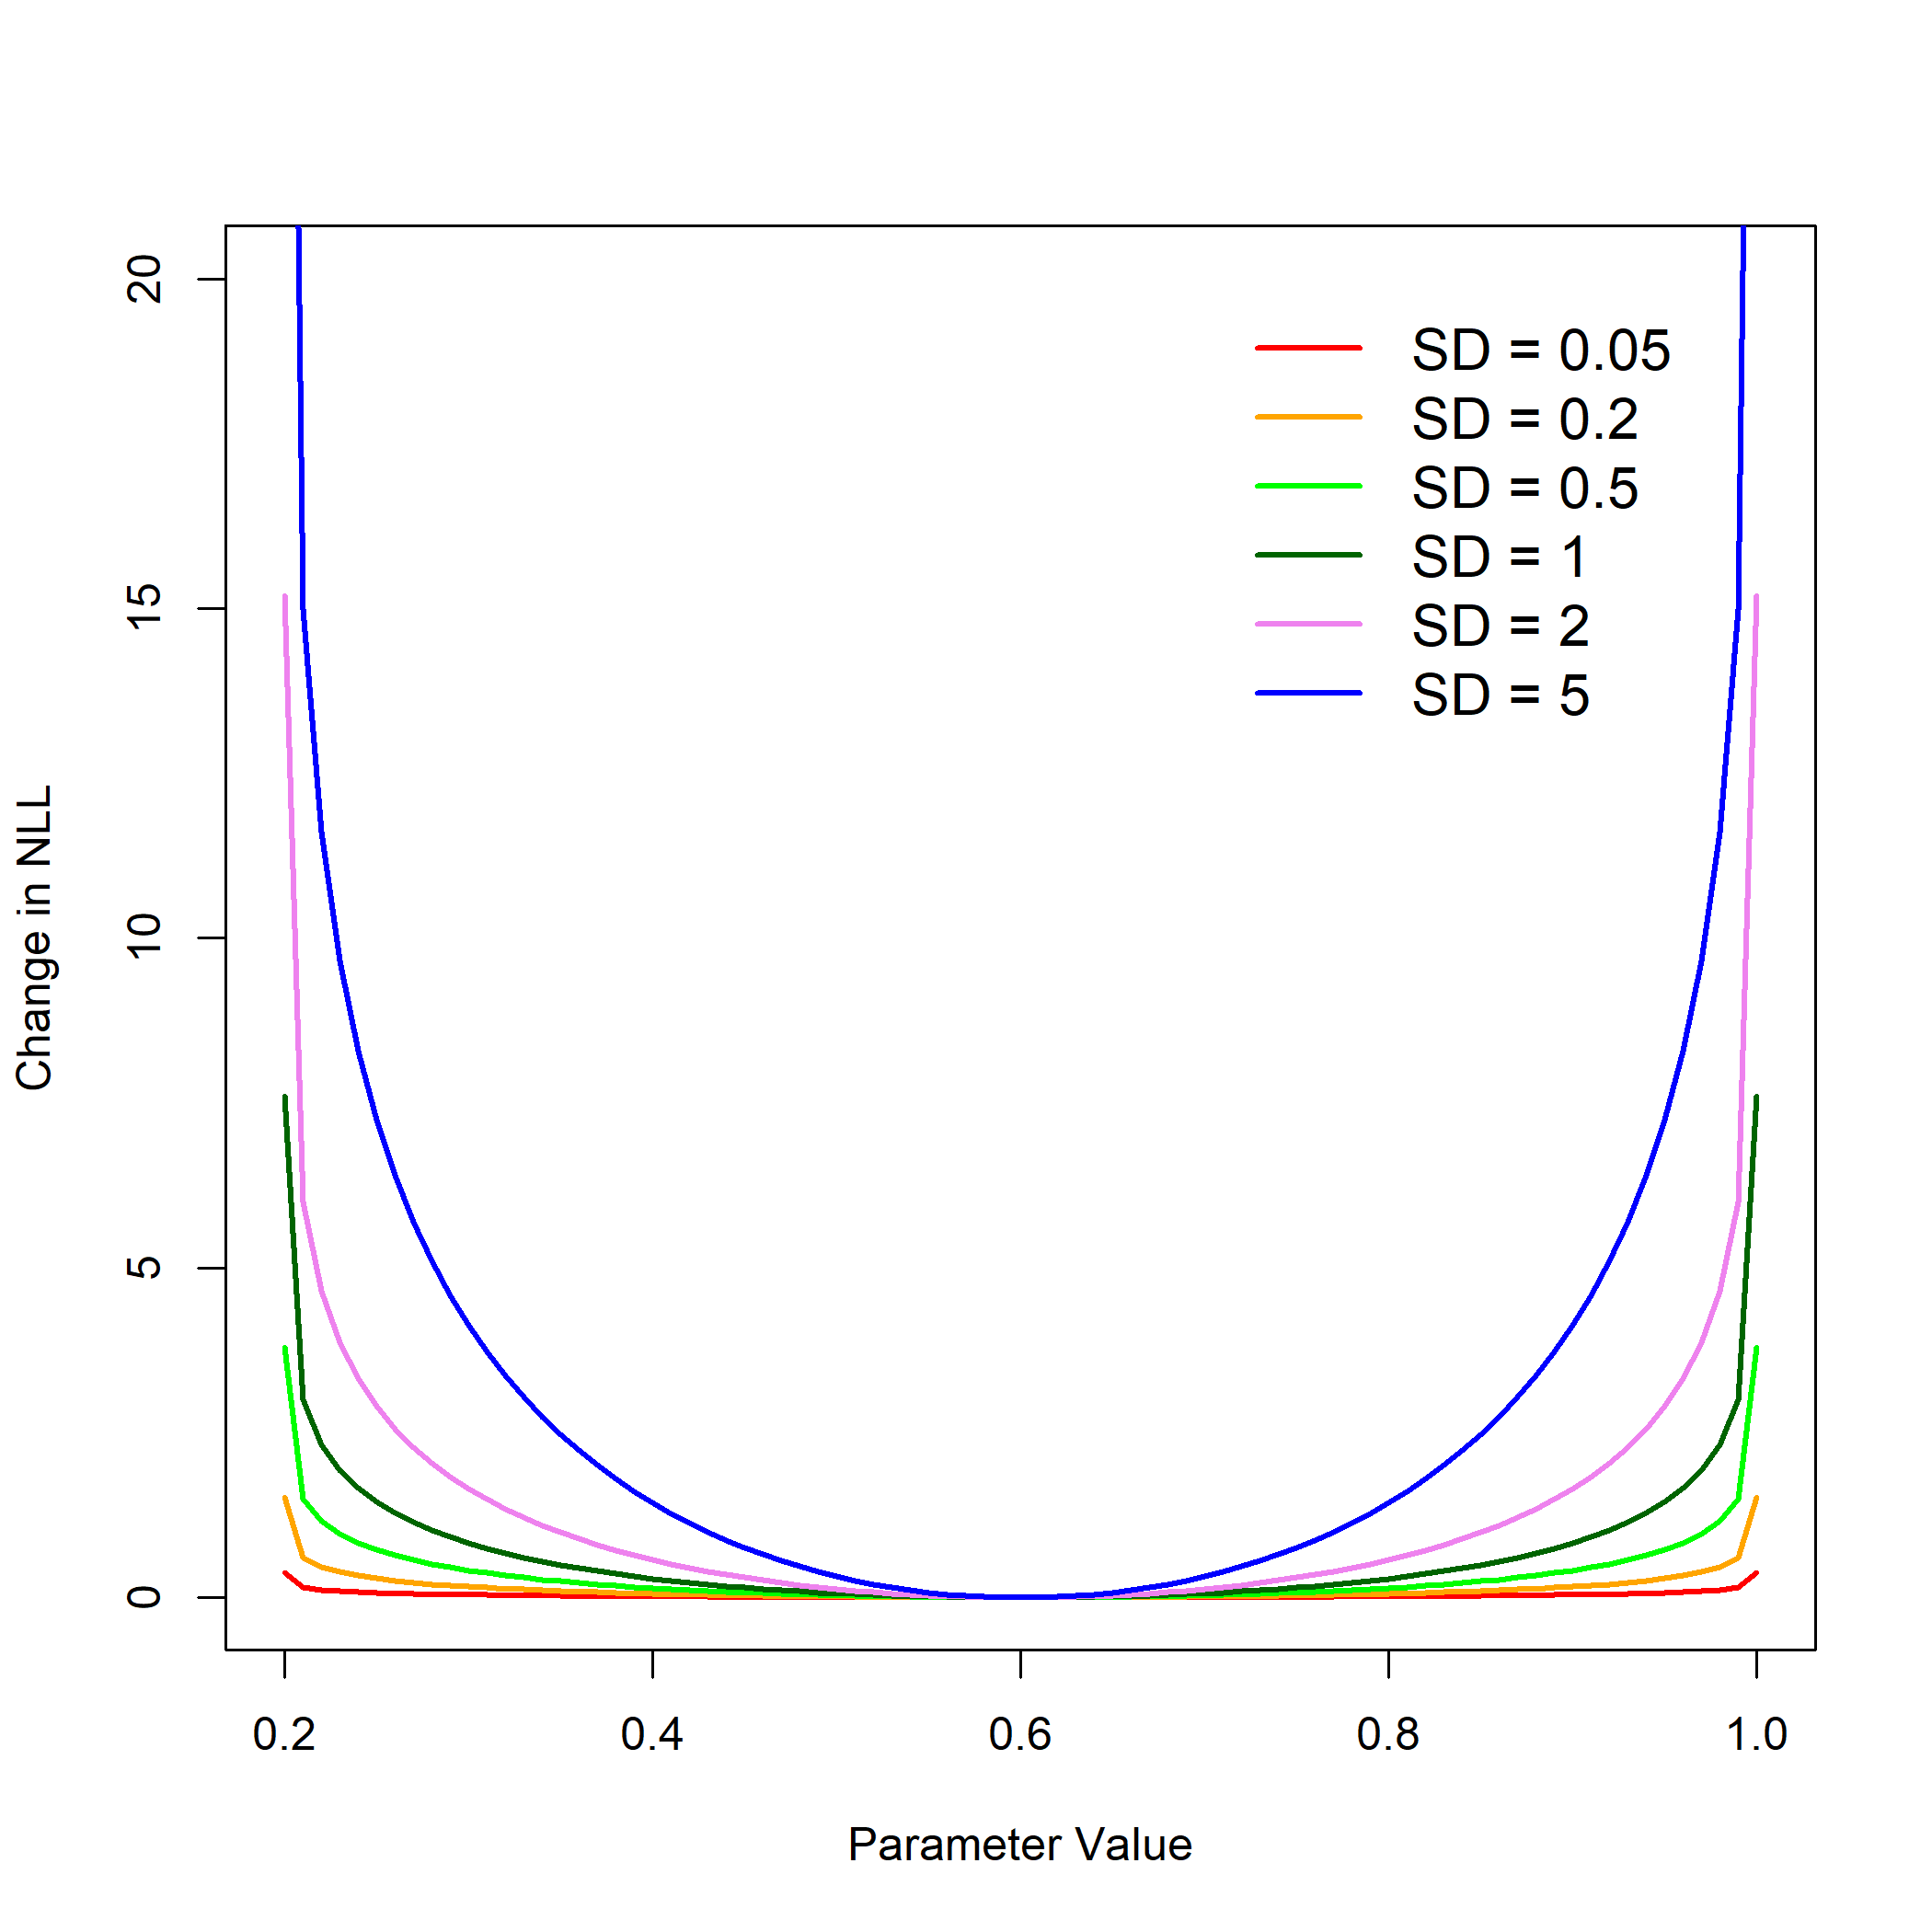
\includegraphics[scale = 0.6]{SymetricBeta}\\
	\end{center}
	\caption{The shape of the symmetric beta prior across alternative standard deviation values and the change in the negative log-likelihood.}
	\end{figure}	

	
	\item \textbf{Prior Type = 2 = Beta prior}  \\ 
	The definition of $\mu$ is consistent with CASAL's formulation with the $\beta_\text{PR}$ and $\alpha_\text{PR}$ corresponding to the $m$ and $n$ parameters.
	\begin{equation}
		\mu = \frac{P_\text{PR}-P_\text{LB}}{P_\text{UB}-P_\text{LB}} 
	\end{equation}
	\begin{equation}
		\tau  = \frac{(P_\text{PR}-P_\text{LB})(P_\text{UB}-P_\text{PR})}{P_\text{PRSD}^2}-1
	\end{equation}
	\begin{equation}
		\beta_\text{PR}  = \tau \cdot \mu
	\end{equation}
	\begin{equation}
		\alpha_\text{PR} = \tau (1-\mu)
	\end{equation}
	
	\begin{equation}
		\begin{split}
			\text{Prior Likelihood} = & (1 - \beta_\text{PR}) \cdot ln(0.0001 + P_\text{init} - P_\text{LB}) \\
			& + (1 - \alpha_\text{PR}) \cdot ln(0.0001 + P_\text{UB} - P_\text{init}) \\
			& - (1 - \beta_\text{PR}) \cdot ln(0.0001 + P_\text{PR} - P_\text{LB}) \\
			& - (1 - \alpha_\text{PR}) \cdot ln(0.0001 + P_\text{UB} - P_\text{PR})
		\end{split}
	\end{equation}

	%\begin{figure}[h]
	%\begin{center}
	%	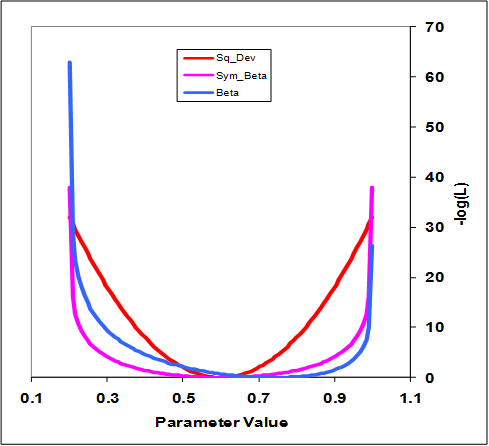
\includegraphics[scale = 0.9]{BetaComparison}\\
	%\end{center}
	%\caption{Comparison of the symmetric beta and the beta prior functions.}
	%\end{figure}	

	
	\item \textbf{Prior Type 3 = Lognormal prior} \\ 
	Note that this is undefined for $p <= 0$ so the lower bound on the parameter must be > 0. The prior value is input into the parameter line in natural log space while the initial parameter value is defined in normal space (e.g., init = 0.20, prior = -1.609438).
	\begin{equation}
		\text{Prior Likelihood} = \frac{1}{2} \left(\frac{ln(P_\text{init})-P_\text{PR}}{P_\text{PRSD}}\right)^2
	\end{equation}
	
	\item \textbf{Prior Type 4 = Lognormal prior with bias correction} \\ 
	This option allows the prior mean value to be entered as the ln(mean). Note that this is undefined for $p <= 0$ so the lower bound on the parameter must be > 0.
	\begin{equation}
		\text{Prior Likelihood} = \frac{1}{2} \left(\frac{ln(P_\text{init})-P_\text{PR} + \frac{1}{2}{P_\text{PRSD}}^2}{P_\text{PRSD}}\right)^2
	\end{equation}
	
	\item \textbf{Prior Type 5 = Gamma prior} \\ 
	The lower bound should be 0 or greater.
	\begin{equation}
		\text{scale} = \frac{{P_\text{PRSD}}^2}{P_\text{PR}}
	\end{equation}
	\begin{equation}
		\text{shape} = \frac{P_\text{PR}}{\text{scale}}
	\end{equation}
	\begin{equation}
		\text{Prior Likelihood} = -\text{shape} \cdot ln(\text{scale}) - ln\big(\Gamma(\text{shape})\big) + (\text{shape} - 1) \cdot ln(P_\text{init}) - \frac{P_\text{init}}{\text{scale}}
	\end{equation}
	
	\item \textbf{Prior Type 6 = Normal prior} \\ 
	Note that this function is independent of the parameter bounds.
	\begin{equation}
		\text{Prior Likelihood} = \frac{1}{2} \left(\frac{P_\text{init} - P_\text{PR}}{P_\text{PRSD}}\right)^2
	\end{equation}
\end{itemize}

%=========Forecast Module
\hypertarget{appendB}{}
\subsection{Forecast Module: Benchmark and Forecasting Calculations}
\label{sec:forecast}

Stock Synthesis v.3.20 introduced substantial upgrades to the benchmark and forecast module. The general intent was to make the forecast outputs more consistent with the requirement to set catch limits that have a known probability of exceeding the overfishing limit. In addition, this upgrade addressed several inadequacies with the previous module, including:

\begin{itemize}
	\item The average selectivity and relative F was the same for the benchmark and the forecast calculations;
	\item The biology-at-age in endyr+1 was used as the biology for the benchmark, but biology-at-age propagated forward in the forecast if there was time-varying growth;
	\item The forecast module had a inefficient approach to calculation of overfishing limit (OFL) conditioned on previously catching ABC;
	\item The forecast module implementation of catch caps was incomplete and applied some caps on a seasonally, rather than the more logical annual basis;
	\item The Fmult scalar for fishing intensity presented a confusing concept for many users;
	\item No provision for specification of catch allocation among fleets;
	\item The forecast allowed for a blend of fixed input catches and catches calculated from target F; this is not optimal for calculation of the variance of F conditioned on a catch policy that sets annual catch limits (ACLs).
\end{itemize}

The v.3.20 module addressed these issues by:
\begin{itemize}
	\item Providing for unique specification of a range of years from which to calculate average selectivity for benchmark, average selectivity for forecast, relative F for benchmark, and relative F for forecast;
	\item Create a new specification for the range of years over which to average size-at-age and fecundity-at-age for the benchmark calculation. In a setup with time-varying growth, it may make sense to do this over the entire range of years in the time series. Note that some additional quantities still use their endyr values, notably the migration rates and the allocation of recruitments among areas. This will be addressed shortly;
	\item Create a multiple pass approach that rectifies the OFL calculation;
	\item Improve the specification of catch caps and implement specification of catch allocations so that there can be an annual cap for each fleet, an annual cap for each area, and an annual allocation among groups of fleets (e.g., all recreational fleets vs. all commercial fleets);
	\item Introduce capability to have implementation error in the forecast catch (single value applied to all fleets in all seasons of the year).
\end{itemize}

\myparagraph{Multiple Pass Forecast}
The most complicated aspect of the changes is with regard to the multiple pass aspect of the forecast.  This multiple pass approach is needed to calculate both OFL and ABC in a single model run. More importantly, the multiple passes are needed in order to mimic the actual sequence of assessment-management action - catch over a multi-year period. The first pass calculates OFL based on catching OFL each year, so presents the absolute maximum upper limit to catches. The second pass forecasts a catch based on a harvest policy, then applies catch caps and allocations, then updates the F's to match these catches. In the third pass, stochastic recruitment and catch implementation error are implemented and SS3 calculates the F that would be needed in order to catch the adjusted catch amount previously calculated in the second pass. With this approach, SS3 is able to produce improved estimates of the probability that F would exceed the overfishing F. In effect it is the complement of the P* approach. Rather than the P* approach that calculates the stream of annual catches that would have an annual probability of F>Flimit, SS3 calculates the expected time series of P* that would result from a specified harvest policy implemented as a buffer between Ftarget and Flimit.

The sequence of multiple forecast passes is as follows:
\begin{enumerate}
	\item Pass 1 (a.k.a. Fcast\_Loop1)
	\begin{enumerate}
		\item Loop Years
		\begin{enumerate}
			\item SubLoop (a.k.a. ABC\_Loop) = 1
			\begin{enumerate}
				\item R = f(SSB) with no deviations
				\item F = Flimit
				\item Fixed input catch amounts ignored
				\item No catch adjustments (caps and allocations)
				\item No implementation error
				\item Result: OFL conditioned on catching OFL each year
			\end{enumerate}
		\end{enumerate}
	\end{enumerate}
	\item Pass 2
	\begin{enumerate}
		\item Loop Years
		\begin{enumerate}
			\item SubLoop = 1
			\begin{enumerate}
				\item R = f(SSB) with no deviations
				\item F = Flimit
				\item Fixed input catch amounts ignored
				\item No catch adjustments (caps and allocations)
				\item No implementation error
				\item Result: OFL conditioned on catching ABC previous year. Stored in std\_vector.
			\end{enumerate}
			\item SubLoop = 2
			\begin{enumerate}
				\item R = f(SSB) with no deviations
				\item F = Ftarget to get catch for each fleet in each season
				\item Fixed input catch amounts replace catch from step 2
				\item Catch adjustments (caps and allocations) applied on annual basis (after looping through seasons and and areas within this year). These adjustments utilize the logistic joiner approach so the overall results remain completely differentiable.
				\item No implementation error
				\item Result: ABC as adjusted for caps and allocations
			\end{enumerate}
			\item SubLoop = 3
			\begin{enumerate}
				\item R = f(SSB) with no deviations
				\item Catches from Pass 2 multiplied by the random term for implementation error
				\item F = adjusted to match the catch*error while taking into account the random recruitments. This is most easily visualized in a MCMC context where the recruitment deviation and the implementation error deviations take on non-zero values in each instance. In MLE, because the forecast recruitments and implementation error are estimated parameters with variance, their variance still propagates to the derived quantities in the forecast.
				\item Result: Values for F, SSB, Recruitment, Catch are stored in std-vectors
				\begin{itemize}
					\item In addition, the ratios F/Flimit and SSB/SSBlimit or SSB/SSBtarget are also stored in std\_vectors.
					\item Estimated variance in these ratios allows calculation of annual probability that F > Flimit or B < Blimit. This is essentially the realized P* conditioned on the specified harvest policy.
				\end{itemize}
			\end{enumerate}
		\end{enumerate}
	\end{enumerate}
\end{enumerate}

\myparagraph{Example Effects on Correlations}
An example that illustrates the above process was conducted. The situation was a low M, late-maturing species, so changes are not dramatic. The example conducted a 10 year forecast and examined correlations with derived quantities in the last year of the forecast. This was done once with the full set of 3 passes as described above, and again with only 2 passes and stochastic recruitment occurring in pass 2, rather than 3. This alternative setup is more similar to forecasts done using previous model versions.

\begin{center}
	\begin{longtable}{p{0.4cm} p{2.75cm} p{3cm} p{1cm} p{0.4cm} p{2.75cm} p{2cm} p{1cm}}
		\hline
		 & \multicolumn{3}{l}{2 Forecast Passes with F from} & & \multicolumn{3}{l}{2 Forecast Passes with catch from} \\
		 & \multicolumn{3}{l}{ABC and random recruitment} & & \multicolumn{3}{l}{target F and equilibrium recruitment} \\
		\hline
		 & Factor X & Factor Y & Corr & & Factor X & Factor Y & Corr \\
		\hline
		A1 & F 2011 & RecrDev 2002 & -0.126 & A2 & F 2011 & RecrDev 2002 & 0.090 \\
		B1 & F 2011 & Recr 2002 & 0.312 & B2 & F 2011 & Recr 2002 & 0.518 \\
		C1 & ForeCatch 2011 & RecrDev 2002 & 0.000 & C2 & ForeCatch 2011 & RecrDev 2002 & 0.129 \\
		D1 & ForeCatch 2011 & Recr 2002 & 0.455 & D2 & Forecatch 2011 & Recr 2002 & 0.555 \\
		\hline		
	\end{longtable}
\end{center}

Correlation A2 shows a small positive correlation between the recruitment deviation in 2002 and the F in 2011. This is probably due to the fact that a positive deviation in recruitment in 2002 will reduce the chances that the biomass in 2011 will be below the inflection point in the control rule. This occurs because in calculating catch from F, the model effectively ``knows'' the future recruitments. I predict that this B1 correlation would be near zero if there was no inflection in the control rule.

Correlation A1 shows this turning into a negative correlation. This is because the future catches are first calculated from equilibrium recruitment, then when random recruitments are implemented, a positive recruitment deviation will cause a negative deviation in the F needed to catch that now ``fixed'' amount of future catch.

Correlations B1 and B2 are in terms of absolute recruitment, not recruitment deviation. Now overall model conditions that cause a higher absolute recruitment level will also result in a higher forecast level. No surprise there, and the correlation is stronger when variance is based on catch is calculated from F (B2).

Correlation C2 shows a positive correlation between recruitment deviation in 2002 and forecast catch in 2011. However, correlation C1 is 0.0 because the forecast catch in 2011 is set based on equilibrium recruitment and is not influenced by the recruitment deviations.

\myparagraph{Future Work}
\begin{itemize}
	\item More testing with high M, rapid turnover conditions
	\item Testing without inflection in control rule
	\item Consider separating implementation error into a pass \#4 so results will more clearly show effect of assessment uncertainty separate from implementation uncertainty
	\item Consider adding a random ``assessment'' error which essentially is a random variable that scales population abundance before passing into the forecast stage. Complication is figuring out how to link it to the correlated error in the benchmark quantities
	\item Because all of these calculations occur only in the standard deviation phase (sdphase) or the MCMC evaluation (mceval) phase, it would be feasible for mceval calls to add an additional pass that is implemented many times and in which random forecast recruitment draws are made.
	\item Factors like selectivity and fleet relative F levels are calculated as an average of these values during the time series. This is internally consistent if these factors do not vary during the time series (although clearly this is a stiff model that will underestimate process variance. However, if these factors do vary over time, then the average used for the forecast will under-represent the variance. A better approach would be to set up the parameters of selectivity as a random process that extends throughout the forecast period, and to update estimated selectivity in each year of the forecast based upon the random realization of these parameters.
\end{itemize}

	


%=========F mortality in SS
\subsection{Fishing Mortality in Stock Synthesis}

The implementation and reporting of fishing mortality rate, $F$, in SS3 has some aspects that can be confusing.  This description provides an overview of the ways in which $F$ is calculated, used, and reported.  

\myparagraph{Rationale}
Fishery management systems expect to have a measure of annual fishing mortality that describes the intensity of the fishery such that an optimal level of $F$ can be articulated and accountability measures can be invoked if $F$ is too high, e.g., overfishing.  This concept is simple and straightforward if the model is a simple biomass dynamics such that a single annual $F$ value operates on the entirety of a non-age structured population. It also is simple for age-structured models that have a single fishing fleet and knife-edge selectivity beginning at some specified age.

The simplicity of $F$ disappears quickly as models invoke a variety of realistic complexities such as: allowing the $F$ to differ among ages or to be based on size; using a collection of fleets with different $F$ levels and different age patterns for $F$; spreading the population across areas and allowing different fleets with different $F$ among the areas.  An unambiguous measure of annual fishing intensity that represents the cumulative effect of all that complexity has not been defined.  This problem has not been solved with SS3, but some logical alternatives have been made available.

\myparagraph{Nomenclature}
The nomenclature below ignores sex, morphs and areas for simplicity. The quantities associated with $F$ calculations are defined as:

$f$ is fleet.

$t$ is a time step; continuous across years $y$ and seasons $s$; equivalent to year if only 1 season.

$a$ is age.

$C_{t,f}$ is fleet-specific catch in a time step.

$B_{t,f}$ is fleet specific available biomass, e.g., total biomass filtered by fleet-specific age selectivity, $s_{t,f,a}$.

$s_{t,f,a}$ is age-specific selectivity for a fleet. If selectivity is length-specific, then age-specific selectivity is calculated as the dot product across length bins of length selectivity and the normal (or lognormal) distribution of length-at-age.  If selectivity is both length- and age-based, which is an entirely normal concept in SS3, then age selectivity due to length selectivity is calculated first, then multiplied by the direct age selectivity.  This compound age selectivity is used in the mortality calculations and is reported as asel2 in report file.  See appendix to \citet{methotstock2013} for more detail on this.

$F_{t,f}'$ is the apical fishing mortality for a fleet. This means that it is the rate for the age that has selectivity equal to 1.0. If your model is using $F'$s as parameters, then the parameter values are for $F'$.

$F_{t,f,a}$ is age and fleet-specific fishing mortality rate equal to $F_{t,f}' * s_{t,f,a}$. Note that it is possible for no age to have a selectivity equal to 1.0. In this case, $F'$ is still the rate for the hypothetical age that has selectivity equal to 1.0. The reported $F'$ values are not rescaled to be an $F$ for the age with peak selectivity. Users need to take this into account if they are comparing reported $F'$ values to reported vector of $F_{t,f,a}$ values.

$\text{ann}F_y$ is a measure of the total fishing intensity for a year, based on one of several user-specified options (see below).

$F\text{std}_y$ is a standardized measure of the total fishing intensity for a year and is reported in the derived quantities, so variance is calculated for this quantity. See below for how it relates to $annF$.

Terminology and reporting of $\text{ann}F$ and $F\text{std}$ has been slightly revised for clarity in 3.30.15.00 and the description here follows the new conventions.

\myparagraph{$F$ Calculation}
SS3 allows for three approaches to estimate the $F'$ that will match the input values for retained catch. Note that SS3 is calculating the $F'$ to match the retained catch conditional on the fraction of total catch that is retained, e.g., the total catch is partitioned into retained and discarded portions.

\begin{enumerate}
	\item Pope's method decays the numbers-at-age to the middle of the season, calculates a harvest rate for each fleet, $H_{t,f}$, that is the ratio of $C_{t,f}$ to $B_{t,f}$, then decays the survivors to the end of the season. The total mortality, $Z_{t,a}$, from the ratio of survivors to initial numbers, is then calculated. The $Z$ is subsequently used for in-season interpolation to get expected values for observations.
	
	\item $F$ as parameters uses the standard Baranov catch equation and lets ADMB find the $F'$ parameter values that produce the lowest negative log-likelihood, which includes fit to the input catch data. $F$ as parameters method tends to work better than Pope's or hybrid in high $F$ situations because it allows for some lack of fit to catch levels in early iterations and can later improve this fit as it closes in on the best solution.
	
	\item Hybrid $F$ starts by calculating a harvest rate, $H$, using Pope's, then converts these $H$ values, which have units of fractional harvest rate, into an approximate of $F'$ in exponential units, tuning these $F'$ values over a few iterations to get a better match to each fleet's catch.
\end{enumerate}

Items to note:
\begin{itemize}
	\item SS3 includes a permutation on the $F$ as parameters method. In the first few phases, SS3 uses hybrid, then between phases it converts these directly calculated $F'$ values into parameters and proceeds in subsequent phases and MCMC to use the parameter approach. This variation on the parameter method is the recommend approach in high $F$ situations.
	
	\item With Pope's method, the $H$ values are fraction caught, so duration of the season does not matter. Parameter and hybrid treat $F'$ identically and multiply the $F'$ values by season duration (which has units of fraction of a year) as it is used. Each of the $F$ methods ends up with a $Z_{t,f}$ that is used for in-season interpolation.
\end{itemize}

\myparagraph{Relative $F$ and $F$mult}
The $F'$ is fleet-specific, so it is useful to have a concept of relative $F$, $\text{rel}F_f$, among fleets. In SS3, $\text{rel}F_f= F_{t,f}'/\sum_{f}^{}F_{t,f}'$ for a single time period $t$. In the benchmark and forecast routines, SS3 can calculate $\text{rel}F_f$ using $F_{t,f}'$ over a range of years, or the user can input custom $\text{rel}F$ values for benchmark and forecast in the forecast.ss file. Note that in a multi-season model setup, $\text{rel}F_f$ is implemented as $\text{rel}F_{s,f}$ where $s$ is the season. These get multiplied by season duration as they are used.

In the benchmark section of the code, SS3 searches for an $F$mult to achieve various management reference points (often referred to as benchmarks). In this search, SS3 calculates a benchmark $F$ as  $F_{ben,f}' = F\text{mult} * \text{rel}F_f$, then calculates equilibrium yield and spawning biomass per recruit (SPR). SS3 searches for the $F$mult that satisfies the search conditions, first for user-specified SPR, then for user-specified spawning biomass at a management target (B\textsubscript{TGT} or $F_{0.1}$), then for MSY. The resultant benchmark quantities are reported in the derived quantities, but $F$mult and $F_{ben,f}'$ are only reported in the Forecast\_report.sso file. SS3 stores the benchmark $F$mult values so that user can invoke them for the forecast.

\myparagraph{Annual $F$}
The $\text{ann}F$ is a single annual value across all fleets and areas according to F\_report\_units, which is specified by users in the starter file. If there are many fleets, across several areas and with very different selectivity patterns, $\text{ann}F$ can have a complicated relationship to apical $F$. The F\_report\_units specification in the starter.ss file, see example line below, allows user to calculate it using $F'$ directly, use exploitation rate, or be derived from $Z$-at-age.

Example $F$ reporting unit specification in the starter.ss file:

\begin{center}
	\begin{longtable}{p{2cm} p{12cm}}
		\hline
		5 & \# F\_report\_units:\Tstrut\\
		  & 0 = skip; \\
		  & 1 = exploitation(Bio); \\
		  & 2 = exploitation(Num); \\ 
		  & 3 = sum(Frates); \\
		  & 4 = true F for range of ages; \\
		  & 5 = unweighted avg. F for range of ages. \Bstrut\\
		\hline
		3 7 & \# min and max age over which average F will be calculated \Tstrut\Bstrut\\
		\hline
	\end{longtable}
\end{center}

For options 4 and 5 of F\_report\_units, the $F$ is calculated as $Z-M$ where $Z$ is calculated as $ln(N_{t+1,a+1}/N_{t,a})$, thus $Z$ subsumes the effect of $F$.

The ann$F$ is calculated for each year of the estimated time series and of the forecast. Additionally, an ann$F$ is calculated in the benchmark calculations to provide equilibrium values that have the same units as ann$F$ from the time series. In versions previous to 3.30.15, it was labeled inaccurately as $F$std in the output, not ann$F$. For example, in the Management Quantities section of derived quantities prior to 3.30.15, there is a quantity labeled Fstd\_Btgt. This is more accurately labeled as the annual $F$ associated with the biomass target, ann\_F\_Btgt, in 3.30.15.

\myparagraph{$F$std}
$F$std is a single annual value based on ann$F$ and the relationship to ann$F$ is specified by F\_report\_basis in the starter.ss file. The benchmark ann$F$ may be used to rescale the time series of ann$F$s to become a time series of standardized values representing the intensity of fishing, $F$std. The report basis is selected in the starter file as:

\begin{center}
	\begin{longtable}{p{2cm} p{12cm}}
		%\multicolumn{2}{l}{The starter file line:}\\
		\hline
		0 & \# F\_report\_basis: \Tstrut\\
		& 0 = raw F report; \\
		& 1 = F / F\textsubscript{SPR}; \\ 
		& 2 = F / F\textsubscript{MSY}; \\
		& 3 = F / F\textsubscript{BTGT}.\Bstrut\\
		\hline
	\end{longtable}
\end{center}

For example, if user selects option 1, $F$ / $F_\text{SPR}$, the time series of ann$F$ will be divided by each value by the ann$F$ calculated in benchmark.

\myparagraph{Units for Stock Synthesis inputs related to $F$}
Below is a list of items to consider in terms of units for $F$ in SS3:
\begin{itemize}
	\item If F\_ballpark is specified in the control.ss file, its units are the same as ann$F$, so is not fleet-specific.
	
	\item $F$ as parameter values has units of fleet-specific apical $F'$.
	
	\item In the forecast.ss file there is an option to input a vector of rel$F$ values. These are dimensionless and will be rescaled to sum to 1.0.
	
	\item In the forecast.ss file there is an option to specify an $F$ scalar for the forecast.  The units of $F$ scalar are the same as the $F$mult values calculated in benchmark.  There are a full set of options for forecast $F$ scalar that can be selected in the forecast file 
	%(-1 = none; 0 = simple; 1 = F\textsubscript{SPR}; 2 = F\textsubscript{MSY} 3 = F\textsubscript{BTGT} or F\textsubscript{0.1}; 4 = Ave F (uses first-last relative F years); and 5 = input annual F scalar). 
	If the forecast $F$ scalar is set as $F_\text{SPR}$, then SS3 will use SPR\_Fmult calculated in benchmark and reported in Forecast-report.sso.  If user selects the option to input an annual $F$ scalar, option 5, then the value is input on a following line.  Whichever method the user selects for forecast $F$ scalar ($F$mult), SS3 will start the forecast by creating a fleet-specific vector of apical $F$ values from $F$mult*rel$F_f$.
	
	\item Also in the forecast.ss file, the last section of inputs allows for input of time and fleet specific apical $F_{t,f}'$ values that override the basic forecast $F$ specification described above.
\end{itemize}


\pagebreak